\let\negmedspace\undefined
\let\negthickspace\undefined
\documentclass[journal,12pt,onecolumn]{IEEEtran}
\usepackage{cite}
\usepackage{amsmath,amssymb,amsfonts,amsthm}
\usepackage{algorithmic}
\usepackage{graphicx}
\usepackage{textcomp}
\usepackage{xcolor}
\usepackage{txfonts}
\usepackage{listings}
\usepackage{enumitem}
\usepackage{mathtools}
\usepackage{gensymb}
\usepackage[breaklinks=true]{hyperref}
\usepackage{tkz-euclide} % loads  TikZ and tkz-base
\usepackage{listings}
\usepackage{gvv}
%
%\usepackage{setspace}
%\usepackage{gensymb}
%\doublespacing
%\singlespacing

%\usepackage{graphicx}
%\usepackage{amssymb}
%\usepackage{relsize}
%\usepackage[cmex10]{amsmath}
%\usepackage{amsthm}
%\interdisplaylinepenalty=2500
%\savesymbol{iint}
%\usepackage{txfonts}
%\restoresymbol{TXF}{iint}
%\usepackage{wasysym}
%\usepackage{amsthm}
%\usepackage{iithtlc}
%\usepackage{mathrsfs}
%\usepackage{txfonts}
%\usepackage{stfloats}
%\usepackage{bm}
%\usepackage{cite}
%\usepackage{cases}
%\usepackage{subfig}
%\usepackage{xtab}
%\usepackage{longtable}
%\usepackage{multirow}
%\usepackage{algorithm}
%\usepackage{algpseudocode}
%\usepackage{enumitem}
%\usepackage{mathtools}
%\usepackage{tikz}
%\usepackage{circuitikz}
%\usepackage{verbatim}
%\usepackage{tfrupee}
%\usepackage{stmaryrd}
%\usetkzobj{all}
%    \usepackage{color}                                            %%
%    \usepackage{array}                                            %%
%    \usepackage{longtable}                                        %%
%    \usepackage{calc}                                             %%
%    \usepackage{multirow}                                         %%
%    \usepackage{hhline}                                           %%
%    \usepackage{ifthen}                                           %%
  %optionally (for landscape tables embedded in another document): %%
%    \usepackage{lscape}     
%\usepackage{multicol}
%\usepackage{chngcntr}
%\usepackage{enumerate}

%\usepackage{wasysym}
%\documentclass[conference]{IEEEtran}
%\IEEEoverridecommandlockouts
% The preceding line is only needed to identify funding in the first footnote. If that is unneeded, please comment it out.

\newtheorem{theorem}{Theorem}[section]
\newtheorem{problem}{Problem}
\newtheorem{proposition}{Proposition}[section]
\newtheorem{lemma}{Lemma}[section]
\newtheorem{corollary}[theorem]{Corollary}
\newtheorem{example}{Example}[section]
\newtheorem{definition}[problem]{Definition}
%\newtheorem{thm}{Theorem}[section] 
%\newtheorem{defn}[thm]{Definition}
%\newtheorem{algorithm}{Algorithm}[section]
%\newtheorem{cor}{Corollary}
\newcommand{\BEQA}{\begin{eqnarray}}
\newcommand{\EEQA}{\end{eqnarray}}
\newcommand{\define}{\stackrel{\triangle}{=}}
\theoremstyle{remark}
\newtheorem{rem}{Remark}

%\bibliographystyle{ieeetr}
\begin{document}
\parindent 0px

\bibliographystyle{IEEEtran}


\vspace{3cm}

\title{
%	\logo{
Solution to 12.13.4.3
%	}
}
\author{ Aryan Jain - EE22BTECH11011$^{*}$% <-this % stops a space	
}	
%\title{
%	\logo{Matrix Analysis through Octave}{\begin{center}\includegraphics[scale=.24]{tlc}\end{center}}{}{HAMDSP}
%}


% paper title
% can use linebreaks \\ within to get better formatting as desired
%\title{Matrix Analysis through Octave}
%
%
% author names and IEEE memberships
% note positions of commas and nonbreaking spaces ( ~ ) LaTeX will not break
% a structure at a ~ so this keeps an author's name from being broken across
% two lines.
% use \thanks{} to gain access to the first footnote area
% a separate \thanks must be used for each paragraph as LaTeX2e's \thanks
% was not built to handle multiple paragraphs
%

%\author{<-this % stops a space
%\thanks{}}
%}
% note the % following the last \IEEEmembership and also \thanks - 
% these prevent an unwanted space from occurring between the last author name
% and the end of the author line. i.e., if you had this:
% 
% \author{....lastname \thanks{...} \thanks{...} }
%                     ^------------^------------^----Do not want these spaces!
%
% a space would be appended to the last name and could cause every name on that
% line to be shifted left slightly. This is one of those "LaTeX things". For
% instance, "\textbf{A} \textbf{B}" will typeset as "A B" not "AB". To get
% "AB" then you have to do: "\textbf{A}\textbf{B}"
% \thanks is no different in this regard, so shield the last } of each \thanks
% that ends a line with a % and do not let a space in before the next \thanks.
% Spaces after \IEEEmembership other than the last one are OK (and needed) as
% you are supposed to have spaces between the names. For what it is worth,
% this is a minor point as most people would not even notice if the said evil
% space somehow managed to creep in.



% The paper headers
%\markboth{Journal of \LaTeX\ Class Files,~Vol.~6, No.~1, January~2007}%
%{Shell \MakeLowercase{\textit{et al.}}: Bare Demo of IEEEtran.cls for Journals}
% The only time the second header will appear is for the odd numbered pages
% after the title page when using the twoside option.
% 
% *** Note that you probably will NOT want to include the author's ***
% *** name in the headers of peer review papers.                   ***
% You can use \ifCLASSOPTIONpeerreview for conditional compilation here if
% you desire.




% If you want to put a publisher's ID mark on the page you can do it like
% this:
%\IEEEpubid{0000--0000/00\$00.00~\copyright~2007 IEEE}
% Remember, if you use this you must call \IEEEpubidadjcol in the second
% column for its text to clear the IEEEpubid mark.



% make the title area
\maketitle



%\tableofcontents

\bigskip

\renewcommand{\thefigure}{\theenumi}
\renewcommand{\thetable}{\theenumi}
%\renewcommand{\theequation}{\theenumi}

%\begin{abstract}
%%\boldmath
%In this letter, an algorithm for evaluating the exact analytical bit error rate  (BER)  for the piecewise linear (PL) combiner for  multiple relays is presented. Previous results were available only for upto three relays. The algorithm is unique in the sense that  the actual mathematical expressions, that are prohibitively large, need not be explicitly obtained. The diversity gain due to multiple relays is shown through plots of the analytical BER, well supported by simulations. 
%
%\end{abstract}
% IEEEtran.cls defaults to using nonbold math in the Abstract.
% This preserves the distinction between vectors and scalars. However,
% if the journal you are submitting to favors bold math in the abstract,
% then you can use LaTeX's standard command \boldmath at the very start
% of the abstract to achieve this. Many IEEE journals frown on math
% in the abstract anyway.

% Note that keywords are not normally used for peerreview papers.
%\begin{IEEEkeywords}
%Cooperative diversity, decode and forward, piecewise linear
%\end{IEEEkeywords}



% For peer review papers, you can put extra information on the cover
% page as needed:
% \ifCLASSOPTIONpeerreview
% \begin{center} \bfseries EDICS Category: 3-BBND \end{center}
% \fi
%
% For peerreview papers, this IEEEtran command inserts a page break and
% creates the second title. It will be ignored for other modes.
%\IEEEpeerreviewmaketitle
\textbf{Question}:
Let X represent the difference between the number of heads and the number of tails obtained when a coin is tossed 6 times. What are the possible values of X? Also find the Probability distribution of X.
\newline
\solution
\newline
It is given that the coin is tossed 6 times.
\newline
Let $H$ be a random variable which denotes the number of heads,
\begin{align}
      H = \{0,1,2,3,4,5,6\}
\end{align}
Let $T$ be a random variable which denotes the number of tails,
\begin{align}
      T &= 6 - H \\
        &= \{6,5,4,3,2,1,0\}
\end{align}
Let X be a random variable which denotes the absolute value of the difference between the number of heads and number of tails,
\begin{align}  
      X &= |H - T| \\
        &= |H - (6 - H)| \\
        &= |2H - 6| 
\end{align} 
Therefore, X can take values from the set \{0,2,4,6\}.  
\newline
Now we will find the probability distribution of X using the CDF approach,
\newline
The CDF of H is given by:
\begin{align}
F_H(k) &= \pr{H \leq k} \\
       &=   \sum_{i=0}^{k} \pr{H=i} \\ 
       &=   \sum_{i=0}^{k} \frac{\comb{6}{i}}{2^6}
\end{align}
First we will do the analysis for k = 2,4 and 6
\newline
So the CDF of X will be:
\begin{align}
F_X(k) &= \pr{X \leq k} \\
       &= \pr{|2H-6| \leq k} \\
       &= \pr{-k \leq 2H-6 \leq k} \\
       &= \pr{\frac{6-k}{2} \leq H \leq \frac{6+k}{2}} \\
       &= F_H\brak{3+\frac{k}{2}} - F_H\brak{(3-\frac{k}{2})-1} \\
       &= F_H\brak{3+\frac{k}{2}} - F_H\brak{2-\frac{k}{2}}
\end{align}
So the probability distribution of X would be given by:
\begin{align}
p_X(k) &= F_X(k) - F_X(k-1) \\
       &= F_H\brak{3+\frac{k}{2}} - F_H\brak{2-\frac{k}{2}} - F_H\brak{2.5+\frac{k}{2}} + F_H\brak{3.5-\frac{k}{2}} \\
       &= \brak{\sum_{i=0}^{3+\frac{k}{2}} \frac{\comb{6}{i}}{2^6} - \sum_{i=0}^{2.5+\frac{k}{2}} \frac{\comb{6}{i}}{2^6}} + \brak{\sum_{i=0}^{3.5-\frac{k}{2}} \frac{\comb{6}{i}}{2^6} - \sum_{i=0}^{2-\frac{k}{2}} \frac{\comb{6}{i}}{2^6}} \\
       &= \frac{\comb{6}{k}}{2^6} + \frac{\comb{6}{6-k}}{2^6} \\
       &= \frac{\comb{6}{k}}{2^5}   \quad \brak{k = 2,4,6}
\end{align}
Now we will do the analysis for k = 0,
\newline
CDF of X for will be
\begin{align}
F_X(k) &= F_H\brak{\sbrak{3+\frac{k}{2}}} - F_H\brak{\sbrak{3-\frac{k}{2}}}
\end{align}
So the probability distribution of X would be given by:
\begin{align}
p_X(k) &= F_X(k) - F_X(k-1) \\
       &= F_H\brak{\sbrak{3+\frac{k}{2}}} - F_H\brak{\sbrak{3-\frac{k}{2}}} - F_H\brak{\sbrak{2.5+\frac{k}{2}}} + F_H\brak{\sbrak{3.5-\frac{k}{2}}} \\
       &= F_H\brak{3+\sbrak{\frac{k}{2}}} - F_H\brak{3-\sbrak{\frac{k}{2}}} - F_H\brak{2+\sbrak{\frac{k}{2}}} + F_H\brak{3-\sbrak{\frac{k}{2}}} \\
       &= F_H\brak{3+\sbrak{\frac{k}{2}}} - F_H\brak{2+\sbrak{\frac{k}{2}}} \\
       &= \sum_{i=0}^{3+\sbrak{\frac{k}{2}}} \frac{\comb{6}{i}}{2^6} - \sum_{i=0}^{2+\sbrak{\frac{k}{2}}} \frac{\comb{6}{i}}{2^6} \quad \brak{k = 0}
\end{align}
The plot of probability distribution of X is shown below:
\begin{figure}
\centering
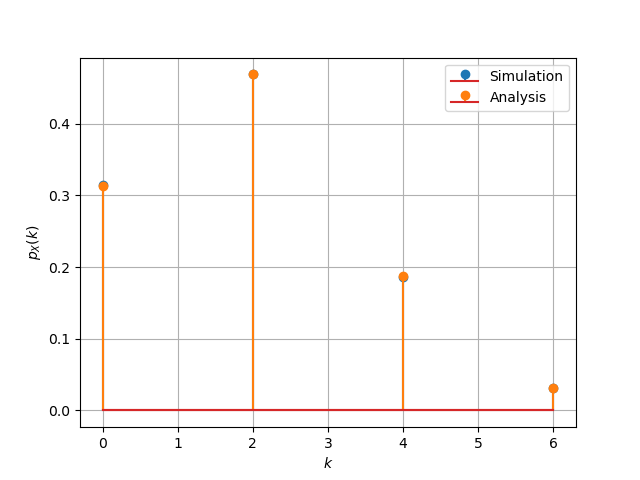
\includegraphics[width=\columnwidth]{./figs/fig.png}
\caption{ PMF of $X$}
\label{tab:ncert/12/13/4/3/}
\end{figure}

\end{document}
